% Copyright 2006 by Till Tantau
%
% This file may be distributed and/or modified
%
% 1. under the LaTeX Project Public License and/or
% 2. under the GNU Free Documentation License.
%
% See the file doc/generic/pgf/licenses/LICENSE for more details.


% \section{Guidelines on Graphics}
\section{绘图准则}

% The present section is not about \pgfname\ or \tikzname, but about general guidelines and principles concerning the creation of graphics for scientific presentations, papers, and books.

本节与\pgfname\ 或\tikzname 无关,而是关于为科学报告、论文和书籍创建图形的一般指导准则或原则。

% The guidelines in this section come from different sources. Many of them are just what I would like to claim is ``common sense'', some reflect my personal experience (though, hopefully, not my personal preferences), some come from books (the bibliography is still missing, sorry) on graphic design and typography. The most influential source  are the brilliant books by Edward Tufte. While I do not agree with everything written in these books, many of Tufte's arguments are so convincing that I decided to repeat them in the following guidelines.

本节中的指导准则来自不同的地方。其中很多都是我想说的``常识'',一些反映了我的个人经验(尽管,希望不只是我个人的喜好),一些来自于平面设计和排版方面的书籍(抱歉,书目还没找到)。最有影响力的资料来源是爱德华·塔夫特的杰出著作。虽然我并不完全同意这些书中所写的一切,但塔夫特的许多论点是如此令人信服,因此我决定在下面的指导准则中重复它们。

% The first thing you should ask yourself when someone presents a bunch of guidelines is: Should I really follow these guidelines? This is an important question, because there are good reasons not to follow general guidelines. The person who set up the guidelines may have had other objectives than you do. For example, a guideline might say ``use the color red for emphasis''. While this guideline makes perfect sense for, say, a presentation using a projector, red ``color'' has the \emph{opposite} effect of ``emphasis'' when printed using a black-and-white printer. Guidelines were almost always set up to address a specific situation. If you are not in this situation, following a guideline can do more harm than good.

当有人提出一系列指导准则时,您应该问自己的第一件事是:我是否真的应该遵循这些指导准则? 这是一个重要的问题,因为有充分的理由不遵循这些准则。 制定准则的人可能有除您之外的其他目标。 例如,一条准则可能会说``用红色表示强调''。 虽然此准则对于使用投影仪进行演示非常有意义,但是当使用黑白打印机进行打印时,红色的``颜色''会具有``强调''的\emph{相反}效果\footnote[1]{译者注:打印出来颜色更浅。}。 准则几乎总是针对特定情况而制定的。如果你不是在这种情况下,那么遵循这些准则可能会弊大于利。

% The second thing you should be aware of is the basic rule of typography is: ``Every rule can be broken, as long as you are \emph{aware} that you are breaking a rule.'' This rule also applies to graphics. Phrased differently, the basic rule states: ``The only mistakes in typography are things done in ignorance.'' When you are aware of a rule and when you decide that breaking the rule has a desirable effect, break the rule.

您应该意识到的第二件事是排版的基本规则:``只要您\emph{意识到}您正在违反规则,那么每个规则都可能被破坏。''该规则也适用于绘图。 基本规则用不同的措词表述:``版式中的唯一错误是未知的东西。''当你意识到一个规则,当你决定打破规则会有更理想的效果,请打破规则。


% \subsection{Planning the Time Needed for the Creation of Graphics}
\subsection{规划创建的图形所需要的时间}

% When you create a paper with numerous graphics, the time needed to create these graphics becomes an important factor. How much time should you calculate for the creation of graphics?

当你创建一篇有大量图形的文章时,创建这些图形所需的时间就成为一个重要的因素。您应该规划多少时间来创建图形?

% As a general rule, assume that a graphic will need as much time to create as would a text of the same length. For example, when I write a paper, I need about one hour per page for the first draft. Later, I need between two and four hours per page for revisions. Thus, I expect to need about half an hour for the creation of \emph{a first draft} of a half page graphic. Later on, I expect another one to two hours before the final graphic is finished.

通常,假设图形创建所需的时间与相同长度的文本所需的时间相同。 例如,当我写论文时,初稿每页大约需要一个小时。 稍后,我需要每页两到四个小时进行修订。 因此,我预计大约需要半小时才能创建半页图形的\emph{初稿}。 稍后,我希望再等一到两个小时才能完成最终图形。

% In many publications, even in good journals, the authors and editors have obviously  invested a lot of time on the text, but seem to have spend about five minutes to create all of the graphics. Graphics often seem to have been added as an ``afterthought'' or look like a screen shot of whatever the authors's statistical software shows them. As will be argued later on, the graphics that programs like \textsc{gnuplot} produce by default are of poor quality.

在许多出版物中,甚至在优质期刊中,作者和编辑者显然都花了大量时间在文本上,但似乎只花了大约五分钟来创建所有图形。 图形似乎经常被认为是``事后思考''的东西,或者看起来就像作者的统计软件显示的屏幕快照一样。 正如稍后将要讨论的那样,默认情况下,像 \textsc{gnuplot} 这样的程序所产生的图形质量很差。

% Creating informative graphics that help the reader and that fit together with the main text is a difficult, lengthy process.

创建有助于读者并与主要内容相适应的信息丰富的图形是一个艰难而漫长的过程。

%
\begin{itemize}
    % \item Treat graphics as first-class citizens of your papers. They deserve as much time and energy as the text does. Indeed, the creation of graphics might deserve \emph{even more} time than the writing of the main text since more attention will be paid to the graphics and they will be looked at first.
    \item 将图形视为你的文章的一等公民。 它们理应需要和文本一样多的时间和精力。 确实,图形的创建可能比主文的写作需要\emph{甚至更多}的时间,因为将更多地关注图形,并且读者首先会关注它们。
    % \item Plan as much time for the creation and revision of a graphic as you would plan for text of the same size.
    \item 与为相同大小的文本的计划一样,计划尽可能多的时间来创建和修改图形。
    % \item Difficult graphics with a high information density may require even more time.
    \item 具有高信息密度的复杂图形可能需要更多时间。
    % \item Very simple graphics will require less time, but most likely you do not want to have ``very simple graphics'' in your paper, anyway; just as you would not like to have a ``very simple text'' of the same size.
    \item 非常简单的图形将需要较少的时间,但是无论如何您很可能不想在纸上创建``非常简单的图形''; 就像您不想拥有相同大小的``非常简单的文字''一样。
\end{itemize}


% \subsection{Workflow for Creating a Graphic}
\subsection{创建图形的工作流程}

% When you write a (scientific) paper, you will most likely follow the following pattern: You have some results/ideas that you would like to report about. The creation of the paper will typically start with compiling a rough outline. Then, the different sections are filled with text to create a first draft. This draft is then revised repeatedly until, often after substantial revision, a final paper results. In a good journal paper there is typically not be a single sentence that has survived unmodified from the first draft.

撰写(科学)论文时,您很可能会遵循以下模式:您有一些要研究的结果或想法。 论文的创建通常从编写一个粗略的轮廓开始。 然后,在不同部分填充文本以完成第一稿。 然后对该草案进行反复修订,直到经常进行实质性修订后才得出最终文件。 在一份好的期刊论文中,通常不会有一个句子从初稿起就没有改变。

% Creating a graphics follows the same pattern:

创建图形遵循相同的模式:

%
\begin{itemize}
    % \item Decide on what the graphic should communicate. Make this a conscious decision, that is, determine ``What is the graphic supposed to tell the reader?''
    \item 决定图表应该传达什么。让这成为一个有意识的决定,也就是说,决定``这个图形要告诉读者什么?''
    % \item Create an ``outline'', that is, the rough overall ``shape'' of the graphic, containing the most crucial elements. Often, it is useful to do this using pencil and paper.
    \item 创建一个``轮廓'',即图形的粗略整体``形状'',其中包含最关键的元素。 通常,使用铅笔和纸进行此操作很有用。
    % \item Fill out the finer details of the graphic to create a first draft.
    \item 填写图形的详细信息以创建第一稿。
    % \item Revise the graphic repeatedly along with the rest of the paper.
    \item 重复修改图形以及本文的其余部分。
\end{itemize}


% \subsection{Linking Graphics With the Main Text}
\subsection{将图形与正文紧密结合}

% Graphics can be placed at different places in a text. Either, they can be inlined, meaning they are somewhere ``in the middle of the text'' or they can be placed in stand-alone ``figures''. Since printers (the people) like to have their pages ``filled'', (both for aesthetic and economic reasons) stand-alone figures may traditionally be placed on pages in the document far away from the main text that refers to them. \LaTeX\ and \TeX\ tend to encourage this ``drifting away'' of graphics for technical reasons.

图形可以放置在文本的不同位置。 可以内联它们,这意味着它们位于``文本中间''的某个位置,或者可以放置在独立的``图形''环境中。 由于打印机(人们)喜欢``填满''他们的页面,因此传统上(出于美学和经济方面的考虑),独立的图形可能会放置在文档中远离引用它们的主要文本的页面上。 由于技术原因,\LaTeX\ 和\TeX\ 倾向于鼓励图形的这种``漂移''。

% When a graphic is inlined, it will more or less automatically be linked with the main text in the sense that the labels of the graphic will be implicitly explained by the surrounding text. Also, the main text will typically make it clear what the graphic is about and what is shown.

对于内联图形,从某种程度上来说,图形的标签将由周围的文本隐含地解释,它会或多或少地自动与主要文本链接。 同样,正文通常会清楚说明图形的含义和显示的内容。

% Quite differently, a stand-alone figure will often be viewed at a time when the main text that this graphic belongs to either has not yet been read or has been read some time ago. For this reason, you should follow the following guidelines when creating stand-alone figures:

完全不同的是,一个独立的图形通常会在这个图形所属的主要文本还没有被读过或者已经读过一段时间的时候被看到。因此,在创建独立图形时,应该遵循以下指导原则:

%
\begin{itemize}
    % \item Stand-alone figures should have a caption than should make them ``understandable by themselves''.
    
    % For example, suppose a graphic shows an example of the different stages of a quicksort algorithm. Then the figure's caption should, at the very least, inform the reader that ``the figure shows the different stages of the quicksort algorithm introduced on page xyz''. and not just ``Quicksort algorithm''.
    \item 独立的图形应该有一个标题,而不是让读者``自己可以理解''。
    
    例如,假设一张图显示了快速排序算法不同阶段的示例。 然后该图的标题至少应告知读者``该图显示了xyz页上介绍的快速排序算法的不同阶段'',不仅仅是``快速排序算法''。
    % \item A good caption adds as much context information as possible. For example, you could say: ``The figure shows the different stages of the quicksort algorithm introduced on page xyz. In the first line, the pivot element 5 is chosen. This causes\dots'' While this information can also be given in the main text, putting it in the caption will ensure that the context is kept. Do not feel afraid of a 5-line caption. (Your editor may hate you for this. Consider hating them back.)
    \item 一个好的标题会添加尽可能多的上下文信息。 例如,您可以说:``该图显示了xyz页上介绍的快速排序算法的不同阶段。 在第一行中,选择了主元素5。 这会导致 \dots 虽然这些信息也可以在正文中给出,但将其放在标题中将确保上下文被保留。 不要害怕5行的标题。(你的编辑可能会因此而讨厌你,考虑反过来讨厌他们。)
    % \item Reference the graphic in your main text as in ``for an example of quicksort `in action', see Figure~2.1 on page xyz''.
    \item 请在正文中引用图形,如``有关快速排序的实际示例,请参阅第xyz页上的图2.1''。
    % \item Most books on style and typography recommend that you do not use abbreviations as in ``Fig.~2.1'' but write ``Figure~2.1''.

    % The main argument against abbreviations is that ``a period is too valuable to waste it on an abbreviation''. The idea is that a period will make the reader assume that the sentence ends after ``Fig'' and it takes a ``conscious backtracking'' to realize that the sentence did not end after all.

    % The argument in favor of abbreviations is that they save space.

    % Personally, I am not really convinced by either argument. On the one hand, I have not yet seen any hard evidence that abbreviations slow readers down. On the other hand, abbreviating all ``Figure'' by ``Fig.'' is most unlikely to save even a single line in most documents. I avoid abbreviations.
    \item 大多数有关样式和排版的书籍建议您不要使用``Fig.~2.1''的缩写版本,而应写``Figure~2.1''。
    
    反对缩写的主要论点是:``句点很有价值,不能浪费在缩写上''。 这个想法是,句点将使读者认为句子在``Fig''之后结束,并且需要进行``有意识的回溯''才能意识到句子毕竟没有结束。

    支持缩写的观点是它们可以节省空间。

    就个人而言,我并没有真正相信任何一种论点。 一方面,我还没有看到任何确凿的证据表明缩写会使读者放慢速度。 另一方面,在所有文档中均使用``Figure''的缩写版本``Fig''可能性很小。 我尽量避免使用缩写。

\end{itemize}


% \subsection{Consistency Between Graphics and Text}
\subsection{图形和文本之间的一致性}

% Perhaps the most common ``mistake'' people do when creating graphics (remember that a ``mistake'' in design is always just ``ignorance'') is to have a mismatch between the way their graphics look and the way their text looks.

也许人们在创建图形时最常见的``错误''(记住设计中的``错误''始终只是``无知'')是图形外观和文本之间看起来不匹配。

% It is quite common that authors use several different programs for creating the graphics of a paper. An author might produce some plots using \textsc{gnuplot}, a diagram using \textsc{xfig}, and include an |.eps| graphic a coauthor contributed using some unknown program. All these graphics will, most likely, use different line widths, different fonts, and have different sizes. In addition, authors often use options like |[height=5cm]| when including graphics to scale them to some ``nice size''.

作者使用几个不同的程序来创建一篇论文的图形是很常见的。作者可能使用 |gnuplot| 生成一些图,使用 |xfig| 生成一个图,还有一个由共同作者使用一些未知的程序生成 |.eps| 图形。所有这些图形很可能使用不同的线宽、不同的字体和不同的大小。此外,作者经常使用像 |[height=5cm]| 这样的选项,当使用这些图形时,将它们缩放到``合适的大小''。

% If the same approach were taken to writing the main text, every section would be written in a different font at a different size. In some sections all theorems would be underlined, in another they would be printed all in uppercase letters, and in another in red. In addition, the margins would be different on each page. Readers and editors would not tolerate a text if it were written in this fashion, but with graphics they often have to.

如果采用同样的方法来书写正文,那么每个部分都将以不同的字体和不同的大小书写。在某些部分,所有的定理都会加下划线,在另一些部分,它们会全部用大写字母打印,而在另一些部分,它们会用红色。此外,每一页的页边距也不一样。读者和编辑不会容忍以这种方式书写的文本,但他们通常却不得不容忍带有图形的文本。

% To create consistency between graphics and text, stick to the following guidelines:

若要使图形和文本之间保持一致,请遵循以下准则:

%
\begin{itemize}
    % \item Do not scale graphics.

    % This means that when generating graphics using an external program, create them ``at the right size''.
    \item 不要缩放图形。
    
    这意味着在使用外部程序生成图形时,请``以适当的尺寸''创建图形。
    % \item Use the same font(s) both in graphics and the body text.
    \item 在图形和正文中使用相同的字体。
    % \item Use the same line width in text and graphics.

    % The ``line width'' for normal text is the width of the stem of letters like T{}. For \TeX, this is usually $0.4\,\mathrm{pt}$. However, some journals will not accept graphics with a normal line width below $0.5\,\mathrm{pt}$.
    \item 在文本和图形中使用相同的线宽。
    
    普通文本的``线宽''是像T{}这样的字母的主干的宽度。对于\TeX,通常是$0.4\,\mathrm{pt}$。但是,有些期刊不接受正常线宽低于$0.5\,\mathrm{pt}$的图形。

    % \item When using colors, use a consistent color coding in the text and in graphics. For example, if red is supposed to alert the reader to something in the main text, use red also in graphics for important parts of the graphic. If blue is used for structural elements like headlines and section titles, use blue also for structural elements of your graphic.

    % However, graphics may also use a logical intrinsic color coding. For example, no matter what colors you normally use, readers will generally assume, say, that the color green as ``positive, go, ok'' and red as ``alert, warning, action''.
    \item  使用颜色时,请在文本和图形中使用一致的颜色编码。 例如,如果红色应该提醒读者注意正文中的某些内容,则在图形中也将红色用于图形的重要部分。 如果将蓝色用于标题和节标题之类的结构元素,请将蓝色也用于图形的结构元素。

    但是,图形也可以使用逻辑上的固有颜色编码。 例如,无论您通常使用什么颜色,读者通常都会假设绿色是``积极,正常,没问题'',红色是``警告,警告,行动''。
\end{itemize}

% Creating consistency when using different graphic programs is almost impossible. For this reason, you should consider sticking to a single graphics program.

使用不同的图形程序时创建一致性的图形几乎是不可能的。 因此,您应该考虑坚持使用单个图形程序。


% \subsection{Labels in Graphics}
\subsection{图形中的标签}

% Almost all graphics will contain labels, that is, pieces of text that explain parts of the graphics. When placing labels, stick to the following guidelines:

几乎所有图形都将包含标签,即用于解释图形各部分的文本。 放置标签时,请遵循以下准则:

%
\begin{itemize}
    % \item Follow the rule of consistency when placing labels. You should do so in two ways: First, be consistent with the main text, that is, use the same font as the main text also for labels. Second, be consistent between labels, that is, if you format some labels in some particular way, format all labels in this way.
    \item 放置标签时,请遵循一致性规则。 您应该通过两种方式进行操作:首先,与主要文本保持一致,即对标签也使用与主文本相同的字体。 其次,标签之间应保持一致,即,如果以某种特定方式格式化某些标签,则应以这种方式格式化所有标签。
    % \item In addition to using the same fonts in text and graphics, you should also use the same notation. For example, if you write $1/2$ in your main text, also use ``$1/2$'' as labels in graphics, not ``0.5''. A $\pi$ is a ``$\pi$'' and not ``$3.141$''. Finally, $\mathrm e^{-\mathrm i \pi}$ is ``$\mathrm e^{-\mathrm i \pi}$'', not ``$-1$'', let alone ``-1''.
    \item 除了在文本和图形中使用相同的字体外,还应该使用相同的符号。 例如,如果您在主文本中写入$1/2$,则还应使用``$1/2$''作为图形中的标签,而不是``0.5''。$\pi$是``$\pi $''而不是``$3.141$''。最后,$\mathrm e^{-\mathrm i \pi}$是``$\mathrm e^{-\mathrm i \pi}$'',而不是``$-1$'',更不用说``-1''了。
    % \item Labels should be legible. They should not only have a reasonably large size, they also should not be obscured by lines or other text. This also applies to labels of lines and text \emph{behind} the labels.
    \item 标签应清晰易读。 它们不仅应具有较大的尺寸,而且也不应被线条或其他文本遮盖。 这也适用于行标签和标签\emph{后面}的文本。
    % \item Labels should be ``in  place''. Whenever there is enough space, labels should be placed next to the thing they label. Only if necessary, add a (subdued) line from the label to the labeled object. Try to avoid labels that only reference explanations in external legends. Reader have to jump back and forth between the explanation and the object that is described.
    \item 标签应放在``适当位置''。 只要有足够的空间,标签就应该放在它们所标记的对象旁边。 只要在必要的时候,才在标签和它们标记的对象用一条(浅色的)的线连接起来。尽量避免只参考外部说明的标签。读者不得不在解释和被描述的对象之间来回跳跃。
    % \item Consider subduing ``unimportant'' labels using, for example, a gray color. This will keep the focus on the actual graphic.
    \item 考虑使用例如灰色来排版``无关紧要''的标签。 这将使读者的焦点集中在实际的图形上。
\end{itemize}


% \subsection{Plots and Charts}
\subsection{图表}

% One of the most frequent kind of graphics, especially in scientific papers, are \emph{plots}. They come in a large variety, including simple line plots, parametric plots, three dimensional plots, pie charts, and many more. 

\emph{图表}是最常见的一种图形,尤其是在科学论文中。它们种类繁多,包括简单的折线图,参数图,三维图,饼图等。

% Unfortunately, plots are notoriously hard to get right. Partly, the default settings of programs like \textsc{gnuplot} or Excel are to blame for this since these programs make it very convenient to create bad plots.

不幸的是,众所周知,图表很难弄对。 部分原因是因为 |gnuplot| 或Excel之类的程序的默认设置,因为这些程序使创建劣质图表非常方便。

% The first question you should ask yourself when creating a plot is: Are there enough data points to merit a plot? If the answer is ``not really'', use a table.

创建图时您应该问自己的第一个问题是:是否有足够的数据点可用于绘制图? 如果答案是``否定的'',请使用表格。

% A typical situation where a plot is unnecessary is when people present a few numbers in a bar diagram. Here is a real-life example: At the end of a seminar a lecturer asked the participants for feedback. Of the 50 participants, 30 returned the feedback form. According to the feedback, three participants considered the seminar ``very good'', nine considered it ``good'', ten ``ok'', eight ``bad'', and no one thought that the seminar was ``very bad''.

不需要绘图的典型情况是人们在条形图中显示一些数字。 这是一个真实的示例:在研讨会结束时,一位讲师要求参与者提供反馈。 在50位参与者中,有30位提交了反馈表。 根据反馈,三位参与者认为研讨会``非常好'',九位认为是``好'',十位``还好'',八位``一般'',没有人认为研讨会``非常差''。

% A simple way of summing up this information is the following table:

下表是汇总这些信息的一种简单方法:

\medskip
\begin{tabular}{lp{3.75cm}r}
  % \emph{Rating given} & \raggedright\emph{Participants (out of 50) who gave this rating} & \emph{Percentage} \\[1.75em]
  \emph{给出的评分} & \raggedright\emph{给予此评分的参与者(共50个)} & \emph{百分比} \\[1.75em]
  % ``very good'' & \hfil\hphantom{0}3\hfil & \hphantom{0}6\% \\
  % ``good'' & \hfil\hphantom{0}9\hfil & 18\% \\
  % ``ok'' & \hfil10\hfil & 20\% \\
  % ``bad'' & \hfil\hphantom{0}8\hfil & 16\% \\
  % ``very bad'' & \hfil\hphantom{0}0\hfil & \hphantom{0}0\% \\[2mm]
  % none & \hfil20\hfil & 40\% \\
  ``非常好'' & \hfil\hphantom{0}3\hfil & \hphantom{0}6\% \\
  ``好'' & \hfil\hphantom{0}9\hfil & 18\% \\
  ``一般'' & \hfil10\hfil & 20\% \\
  ``差'' & \hfil\hphantom{0}8\hfil & 16\% \\
  ``非常差'' & \hfil\hphantom{0}0\hfil & \hphantom{0}0\% \\[2mm]
  未评分 & \hfil20\hfil & 40\% \\
\end{tabular}

\bigskip
% What the lecturer did was to visualize the data using a 3D bar diagram. It looked like this (except that in reality the numbers where typeset using some extremely low-resolution bitmap font and were near-unreadable):

讲师所做的就是使用3D条形图将数据可视化。 它看起来像这样(实际上,数字是使用某些分辨率非常低的位图字体进行排版的,几乎无法读取):

\bigskip
\par
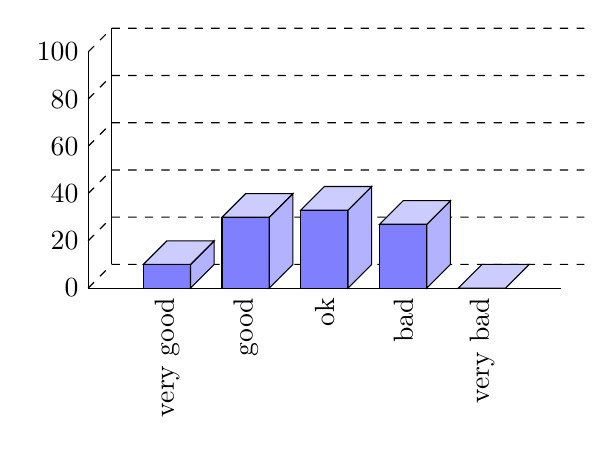
\begin{tikzpicture}[y=0.03cm,z=3mm]
  \foreach \y in {0,20,40,60,80,100}
    \draw[dashed] (0,\y,0) node[left] {\y} -- (0,\y,1)  -- (6,\y,1);

  \draw (0,0,0) -- (0,100,0)  (0,0,1) -- (0,100,1);
  \draw (0,0,0) -- (6,0,0);

  \foreach \x/\xtext/\height in {1/very good/10,2/good/30,3/ok/33,4/bad/27,5/very bad/0}
  {
    \draw (\x,0) node[rotate=90,anchor=east] {\xtext};

    \begin{scope}[xshift=\x cm]

    \filldraw[fill=blue!50] (-.3,0,0) rectangle (.3,\height,0);
    \filldraw[fill=blue!30] (.3,0,0) -- (.3,0,1) -- (.3,\height,1) -- (.3,\height,0) --cycle;
    \filldraw[fill=blue!20] (-.3,\height,0) -- (.3,\height,0) --
    (.3,\height,1) -- (-.3,\height,1) --cycle;
    \end{scope}
  }
\end{tikzpicture}
\bigskip

% Both the table and the ``plot'' have about the same size. If your first thought is ``the graphic looks nicer than the table'', try to answer the following questions based on the information in the table or in the graphic:

表和``图''的大小大致相同。 如果您首先想到的是``图形看起来比表格更好'',请尝试根据表格或图形中的信息回答以下问题:

%
\begin{enumerate}
    % \item How many participants where there?
    \item 总共有多少参与者?
    % \item How many participants returned the feedback form?
    \item 有多少参与者退回了反馈表?
    % \item What percentage of the participants returned the feedback form?
    \item 百分之几的参与者返回了反馈表?
    % \item How many participants checked ``very good''?
    \item 有多少参与者的评价``非常好''?
    % \item What percentage out of all participants checked ``very good''?
    \item 在所有参与者中,有多少百分比表示``非常好''?
    % \item Did more than a quarter of the participants check ``bad'' or ``very bad''?
    \item 是否有超过四分之一的参与者检查``差''或``非常差''?
    % \item What percentage of the participants that returned the form checked ``very good''?
    \item 提交了反馈表的参与者中有百分之多少表示``非常好''?
\end{enumerate}

% Sadly, the graphic does not allow us to answer \emph{a single one of these questions}. The table answers all of them directly, except for the last one. In essence, the information density of the graphic is very close to zero. The table has a much higher information density; despite the fact that it uses quite a lot of white space to present a few numbers. Here is the list of things that went wrong with the 3D-bar diagram:

可悲的是,该图形不允许我们回答\emph{这些问题中的任何一个}。 该表直接回答所有问题,除了最后一个。 本质上,图形的信息密度非常接近零。 该表具有更高的信息密度; 尽管它使用大量空白来表示一些数字。 以下是3D条形图出现问题的列表:

%
\begin{itemize}
    % \item The whole graphic is dominated by irritating background lines.
    \item 整个图形以令人讨厌的背景线为主。
    % \item It is not clear what the numbers at the left mean; presumably percentages, but it might also be the absolute number of participants.
    \item 目前尚不清楚左边的数字是什么意思。 大概是百分比,但也可能是参与者的绝对人数。
    % \item The labels at the bottom are rotated, making them hard to read.

    % (In the real presentation that I saw, the text was rendered at a very low resolution with about 10 by 6 pixels per letter with wrong kerning, making the rotated text almost impossible to read.)
    \item 底部的标签被旋转,使其难以阅读。
    
    (在我看到的真实演示中,文本的分辨率非常低,每个字母大约 10 × 6 像素,而且字距错误,使得旋转后的文本几乎无法读取。)
    % \item The third dimension adds complexity to the graphic without adding information.
    \item 第三维在不添加信息的情况下增加了图形的复杂性。
    % \item The three dimensional setup makes it much harder to gauge the height of the bars correctly. Consider the ``bad'' bar. It the number this bar stands for more than 20 or less? While the front of the bar is below the 20 line, the back of the bar (which counts) is above.
    \item 三维设置使正确度量柱的高度变得十分困难。 考虑一下``差''这一柱。 这一条代表的数字是否是大于或等于20? 柱状图的前部在20以下,而柱状图的后部确在其在上方。
    % \item It is impossible to tell which  numbers are represented by the bars. Thus, the bars needlessly hide the information these bars are all about.
    \item 我们无法分辨这些柱状图代表的是哪些数字。因此,这些柱不必要地隐藏了这些柱所包含的所有信息。
    % \item What do the bar heights add up to? Is it 100\% or 60\%?
    \item 杆高加起来是多少? 是100%还是60%?
    % \item Does the bar for ``very bad'' represent 0 or~1?
    \item ``非常差''柱代表0还是1?
    % \item Why are the bars blue?
    \item 为什么柱是蓝色的?
\end{itemize}

% You might argue that in the example the exact numbers are not important for the graphic. The important things is the ``message'', which is that there are more ``very good'' and ``good'' ratings than ``bad'' and ``very bad''. However, to convey this message either use a sentence that says so or use a graphic that conveys this message more clearly:

你可能会说,在这个例子中,确切的数字对图表并不重要。重要的是``信息'',即``非常好''和``好''的评级要多于``差''和``非常差''的评级。但是,要传达这一信息,可以用句子来表达,也可以用图表来更清楚地表达:
\medskip
\par
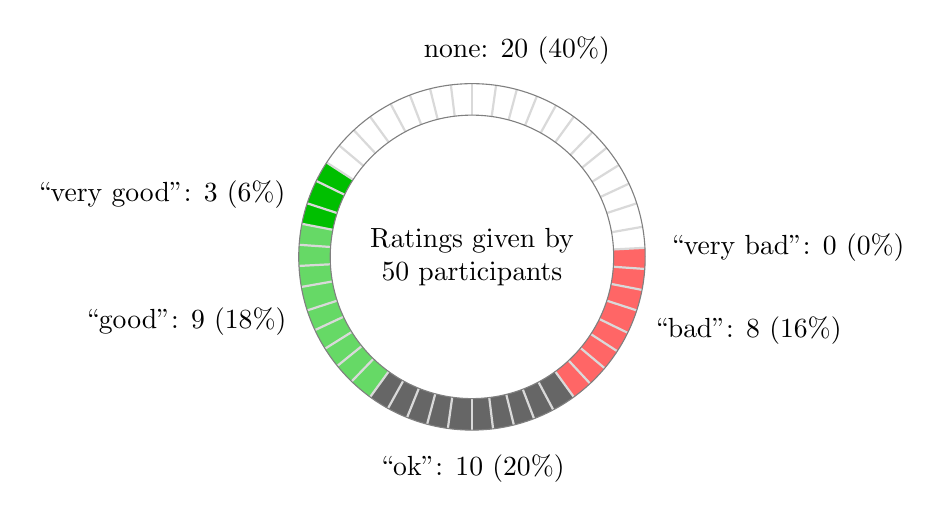
\begin{tikzpicture}
  \colorlet{good}{green!75!black}
  \colorlet{bad}{red}
  \colorlet{neutral}{black!60}
  \colorlet{none}{white}

  \node[align=center,text width=3cm]{Ratings given by 50~participants};

  \begin{scope}[line width=4mm,rotate=270]
    \draw[good]          (-123:2cm) arc (-123:-101:2cm);
    \draw[good!60!white] (-36:2cm) arc (-36:-101:2cm);
    \draw[neutral]       (-36:2cm) arc (-36:36:2cm);
    \draw[bad!60!white]  (36:2cm)  arc (36:93:2cm);

    \newcount\mycount
    \foreach \angle in {0,72,...,3599}
    {
      \mycount=\angle\relax
      \divide\mycount by 10\relax
      \draw[black!15,thick] (\the\mycount:18mm) -- (\the\mycount:22mm);
    }

    \draw (0:2.2cm) node[below] {``ok'': 10 (20\%)};
    \draw (165:2.2cm) node[above] {none: 20 (40\%)};
    \draw (-111:2.2cm) node[left] {``very good'': 3 (6\%)};
    \draw (-68:2.2cm) node[left] {``good'': 9 (18\%)};
    \draw (65:2.2cm) node[right] {``bad'': 8 (16\%)};
    \draw (93:2.2cm) node[right] {``very bad'': 0 (0\%)};
  \end{scope}
  \draw[gray] (0,0) circle (2.2cm) circle (1.8cm);
\end{tikzpicture}

\bigskip
% The above graphic has about the same information density as the table (about the same size and the same numbers are shown). In addition, one can directly ``see'' that there are more good or very good ratings than bad ones. One can also ``see'' that the number of people who gave no rating at all is not negligible, which is quite common for feedback forms.

上面的图形与表格具有大约相同的信息密度(显示的大小和数字大致相同)。 此外,人们可以直接``看到''好的评级比不良评级更高。 人们也可以``看到'',根本没有给出评分的人数是微不足道的,这对于反馈表来说是很普遍的。

% Charts are not always a good idea. Let us look at an example that I redrew from a pie chart in \emph{Die Zeit}, June 4th, 2005:

图表并非总是一个好主意。 让我们看一个我从2005年6月4日\emph{时代周刊}中的饼图的一个重新绘制的示例:

\bigskip
\par
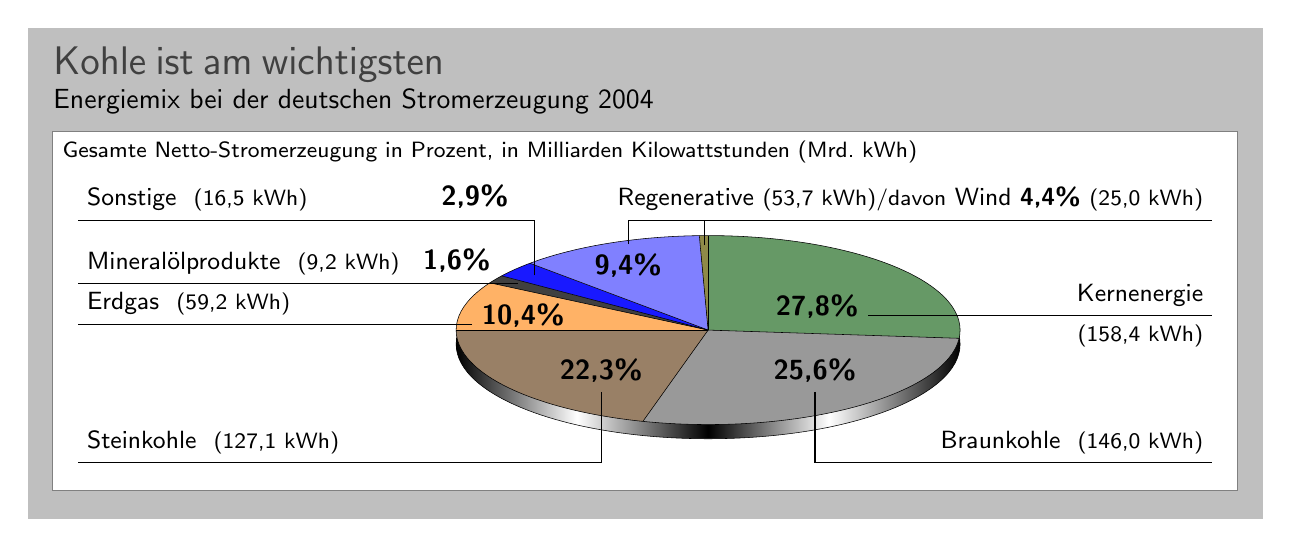
\begin{tikzpicture}
  \begin{scope}[xscale=3.2,yscale=1.2]

    \sffamily
    \coordinate (right border) at (2.0cm,-1.7cm);
    \coordinate (left border)  at (-2.5cm,2.1cm);

    \fill[black!25] ([xshift=-2mm,yshift=1.1cm]left border) rectangle ([xshift=2mm,yshift=-.3cm]right border);

    \node[below right,text width=10cm,inner sep=0pt] at ([yshift=.9cm,xshift=-1mm]left border)
    { {\color{black!75} \Large Kohle ist am wichtigsten}\\
      Energiemix bei der deutschen Stromerzeugung 2004};

    \filldraw[draw=gray,fill=white] ([xshift=-1mm]left border) node[below right,black]
      {\footnotesize Gesamte Netto-Stromerzeugung in Prozent, in Milliarden Kilowattstunden (Mrd.\ kWh)}
      rectangle ([xshift=1mm]right border);

    % The 3D stuff
    \pgfdeclarehorizontalshading{zeit}{100bp}
    {color(0pt)=(black);
      color(25bp)=(black);
      color(37bp)=(white);
      color(50bp)=(black);
      color(62bp)=(white);
      color(75bp)=(black);
      color(100bp)=(black)}

    \shadedraw[very thin,shading=zeit,yshift=-1.5mm] (0,0) circle (1cm);

    \fill[green!20!gray]   (0,0) -- (90:1cm) arc (90:-5:1cm);
    \fill[white!20!gray]   (0,0) -- (-5:1cm) arc (-5:-105:1cm);
    \fill[orange!20!gray]  (0,0) -- (-105:1cm) arc (-105:-180:1cm);
    \fill[orange!60!white] (0,0) -- (180:1cm) arc (180:150:1cm);
    \fill[black!75!white]  (0,0) -- (150:1cm) arc (150:145:1cm);
    \fill[blue!90!white]   (0,0) -- (145:1cm) arc (145:135:1cm);
    \fill[blue!50!white]   (0,0) -- (135:1cm) arc (135:92:1cm);
    \fill[yellow!50!black] (0,0) -- (92:1cm) arc (92:90:1cm);

    \begin{scope}[very thin]
      \draw (0,0) -- (90:1cm);
      \draw (0,0) -- (-5:1cm);
      \draw (0,0) -- (-105:1cm);
      \draw (0,0) -- (-180:1cm);
      \draw (0,0) -- (150:1cm);
      \draw (0,0) -- (145:1cm);
      \draw (0,0) -- (135:1cm);
      \draw (0,0) -- (92:1cm);

      \draw(0,0) circle (1cm);
    \end{scope}

    \node (Regenerative)   at (115:.75cm)  {\bfseries 9,4\%};
    \node (Kernenergie)    at (30:.5cm)   {\bfseries 27,8\%};
    \node (Braunkohle)     at (-45:.6cm)  {\bfseries 25,6\%};
    \node (Steinkohle)     at (-135:.6cm) {\bfseries 22,3\%};
    \node (Erdgas)         at (168:.75cm) {\bfseries 10,4\%};
    \coordinate (Mineral)  at (147:.9cm);
    \coordinate (Sonstige) at (140:.9cm);

    \small
    \draw (Regenerative.north) |- ([yshift=.25cm]Regenerative.north -| right border) coordinate (Regenerative label);
    \draw (91:.9cm) |- (Regenerative label);
    \node[above left] at (Regenerative label) {Regenerative\
      {\footnotesize (53,7 kWh)/davon} Wind \textbf{4,4\%}  \footnotesize (25,0 kWh)};

    \draw (Kernenergie.base east) -- (Kernenergie.base east -| right border) coordinate (Kernenergie label);
    \node[above left] at (Kernenergie label) {Kernenergie};
    \node[below left] at (Kernenergie label) {\footnotesize (158,4 kWh)};

    \draw (Braunkohle.south) |- ([yshift=-.75cm]Braunkohle.south -| right border) coordinate (Braunkohle label);
    \node[above left] at (Braunkohle label) {Braunkohle\ \ \footnotesize (146,0 kWh)};

    \draw (Steinkohle.south) |- ([yshift=-.75cm]Steinkohle.south -| left border) coordinate (Steinkohle label);
    \node[above right] at (Steinkohle label) {Steinkohle\ \ \footnotesize (127,1 kWh)};

    \draw (Erdgas.base west) -- (Erdgas.base west -| left border) coordinate (Erdgas label);
    \node[above right] at (Erdgas label) {Erdgas\ \ \footnotesize (59,2 kWh)};

    \draw (Mineral) -- (Mineral -| left border) coordinate (Mineral label);
    \node[above right] at (Mineral label) {Mineral\"olprodukte\ \
      \footnotesize (9,2 kWh) \  \ \normalsize\textbf{1,6\%}};

    \draw (Sonstige) |- (Regenerative label -| left border) coordinate (Sonstige label);
    \node[above right] at (Sonstige label) {Sonstige\ \
      \footnotesize (16,5 kWh) \hskip1.5cm\
      \normalsize\textbf{2,9\%}};
  \end{scope}
\end{tikzpicture}

% This graphic has been redrawn in \tikzname, but the original looks almost exactly the same.

该图形已用\tikzname 重绘,但原始外观几乎完全相同。

% At first sight, the graphic looks ``nice and informative'', but there are a lot of things that went wrong:

乍一看,该图形看起来``不错且内容丰富'',但是有很多地方出了问题:

%
\begin{itemize}
    % \item The chart is three dimensional. However, the shadings add nothing ``information-wise'', at best, they distract.
    \item 图表是三维的。 但是,阴影没有增加``信息方面''的内容,充其量只能分散注意力。
    % \item In a 3D-pie-chart the relative sizes are very strongly distorted. For example, the area taken up by the gray color of ``Braunkohle'' is larger than the area taken up by the green color of ``Kernenergie'' \emph{despite the fact that the percentage of Braunkohle is less than the percentage of Kernenergie}.
    \item 在3D饼图中,相对大小会非常严重地变形。 例如,灰色的``Braunkohle''占据的面积大于绿色的``Kernenergie''占据的面积,\emph{尽管Braunkohle的百分比小于Kernergye的百分比}。
    % \item The 3D-distortion gets worse for small areas. The area of ``Regenerative'' somewhat larger  than the area of ``Erdgas''. The area of ``Wind'' is slightly smaller than the area of ``Mineral\"olprodukte'' \emph{although the percentage of Wind is nearly three times larger than the percentage of Mineral\"olprodukte.}

    % In the last case, the different sizes are only partly due to distortion. The designer(s) of the original graphic have also made the ``Wind'' slice too small, even taking distortion into account. (Just compare the size of ``Wind'' to ``Regenerative'' in general.)

    \item 3D失真在小区域变得更糟。  ``Regenerative''面积比``Erdgas''面积大。``Wind''的面积略小于``Mineral\"olprodukte''的面积,\emph{(尽管``Wind''的百分比几乎是矿产``Mineral\"olprodukte''的百分比的三倍。}

    在最后一种情况下,不同的大小只是部分上归咎于失真。原图的设计者还把``Wind''的切片做得太小,甚至把失真也考虑进去了。(只要比较一下``Wind''和``Regenerative''的一般大小就可以了。)
    % \item According to its caption, this chart is supposed to inform us that coal was the most important energy source in Germany in 2004. Ignoring the strong distortions caused by the superfluous and misleading 3D-setup, it takes quite a while for this message to get across.

    % Coal as an energy source is split up into two slices: one for ``Steinkohle'' and one for ``Braunkohle'' (two different kinds of coal). When you add them up, you see that the whole lower half of the pie chart is taken up by coal.

    % The two areas for the different kinds of coal are not visually linked at all. Rather, two different colors are used, the labels are on different sides of the graphic. By comparison, ``Regenerative'' and ``Wind'' are very closely linked.
    \item 根据其标题,此图表应该告诉我们,煤炭是2004年德国最重要的能源。忽略了多余和误导性的3D设置所造成的强烈变形,此信息需要花很长时间才能传达出来。
    
    煤炭作为能源分为两部分:一个是``Steinkohle'',另一个是``Braunkohle''(两种不同的煤炭)。 将它们加起来后,您会看到饼图的整个下半部分都被煤炭占据了。

    不同种类的煤炭的两个区域根本没有视觉上的联系。 而是使用两种不同的颜色,标签位于图形的不同侧。 相比之下,``Regenerative''和``Wind''连接更为紧密。
    % \item The color coding of the graphic follows no logical pattern at all. Why is nuclear energy green? Regenerative energy is light blue, ``other sources'' are blue. It seems more like a joke that the area for ``Braunkohle'' (which literally translates to ``brown coal'') is stone gray, while the area for ``Steinkohle'' (which literally translates to ``stone coal'') is brown.
    \item 图形的颜色编码没有遵循任何逻辑模式。为什么核能是绿色的?再生能源是浅蓝色的,``其他能源''是蓝色的。``Braunkohle''(字面意思是``棕色的煤'')的区域是石灰色的,而``Steinkohle''(字面意思是``石煤'')的区域是棕色的,这看起来更像是一个笑话。
    % \item The area with the lightest color is used for ``Erdgas''. This area stands out most because of the brighter color. However, for this chart ``Erdgas'' is not really important at all.
    \item 颜色最亮的区域用于``Erdgas''。 该区域最突出的原因是颜色较亮。 但是,对于这个图表,``Erdgas''一点都不重要。
\end{itemize}
%
% Edward Tufte calls graphics like the above ``chart junk''. (I am happy to announce, however, that \emph{Die Zeit} has stopped using 3D pie charts and their information graphics have got somewhat better.)
%
爱德华·塔夫特(Edward Tufte)将上述图形称为``垃圾图表''。(不过,我很高兴地宣布\emph{时代周刊}已经停止使用3D饼图,并且其信息图也有所改善。)

% Here are a few recommendations that may help you avoid producing chart junk:

以下是一些建议,可以帮助您避免创建垃圾图表:
%
\begin{itemize}
    % \item Do not use 3D pie charts. They are \emph{evil}.
    \item 不要使用3D饼图。它是\emph{邪恶的}。
    % \item Consider using a table instead of a pie chart.
    \item 考虑使用表格而不是饼图。
    % \item Do not apply colors randomly; use them to direct the readers's focus and to group things.
    \item 请勿随机应用颜色;而应用它们来引导读者的注意力并对事物进行分组。
    % \item Do not use background patterns, like a crosshatch or diagonal lines, instead of colors. They distract. Background patterns in information graphics are \emph{evil}.
    \item 请勿使用背景图案(例如交叉线或对角线)代替背景颜色。他们会使读者分心。 信息图中的背景图案是\emph{邪恶的}。
\end{itemize}


% \subsection{Attention and Distraction}
\subsection{注意力和注意力分散}

% Pick up your favorite fiction novel and have a look at a typical page. You will notice that the page is very uniform. Nothing is there to distract the reader while reading; no large headlines, no bold text, no large white areas. Indeed, even when the author does wish to emphasize something, this is done using italic letters. Such letters blend nicely with the main text -- at a distance you will not be able to tell whether a page contains italic letters, but you would notice a single bold word immediately. The reason novels are typeset this way is the following paradigm: Avoid distractions.

挑选您最喜欢的小说,并浏览典型的页面。 您会注意到页面非常统一。 在阅读时,没有什么可以分散读者的注意力。 没有大的标题,没有粗体的文字,没有大的白色区域。 确实,即使作者确实希望强调某些内容,也可以使用斜体字母。 这样的字母与主要文本很好地融合在一起,在一段距离内您将无法分辨页面是否包含斜体字母,但是您会立即注意到一个粗体字。 小说被排版的原因是以下范例:避免分神。

% Good typography (like good organization) is something you do \emph{not} notice. The job of typography is to make reading the text, that is, ``absorbing'' its information content, as effortless as possible. For a novel, readers absorb the content by reading the text line-by-line, as if they were listening to someone telling the story. In this situation anything on the page that distracts the eye from  going quickly and evenly from line to line will make the text harder to read.

好的排版(如好的组织)是您要做到\emph{不}引起注意。 排版的工作是使文本阅读尽可能轻松,即``吸收''其内容。 对于小说来说,读者通过逐行阅读文本来吸收内容,就好像他们在听某人讲故事一样。 在这种情况下,页面上的任何东西都会分散眼睛的注意力,使他们无法快速,均匀地一行一行一行地阅读,这会使文本难以阅读。

% Now, pick up your favorite weekly magazine or newspaper and have a look at a typical page. You will notice that there is quite a lot ``going on'' on the page. Fonts are used at different sizes and in different arrangements, the text is organized in narrow columns, typically interleaved with pictures. The reason magazines are typeset in this way is another paradigm: Steer attention.

现在,选择您喜欢的每周杂志或报纸,然后浏览典型的页面。 您会注意到页面上有很多``正在进行中''。 字体以不同的大小和排列方式使用,文本以窄列组织,通常与图片交错。 杂志以这种方式排版的原因是另一个范例:引导注意力。

% Readers will not read a magazine like a novel. Instead of reading a magazine line-by-line, we use headlines and short abstracts to check whether we want to read a certain article or not. The job of typography is to steer our attention to these abstracts and headlines, first. Once we have decided that we want to read an article, however, we no longer tolerate distractions, which is why the main text of articles is typeset exactly the same way as a novel.

读者不会像小说一样阅读杂志。 与其逐行阅读杂志,不如使用标题和简短摘要来检查我们是否要阅读某篇文章。 排版工作首先是要引起我们对这些摘要和标题的关注。 但是,一旦决定要阅读一篇文章,我们就不再容忍分心,这就是为什么文章的正文排版与小说完全一样的原因。

% The two principles ``avoid distractions'' and ``steer attention'' also apply to graphics. When you design a graphic, you should eliminate everything that will ``distract the eye''. At the same time, you should try to actively help the reader ``through the graphic'' by using fonts/colors/line widths to highlight different parts.

``避免分心''和``引导注意力''这两个原则也适用于图形。 设计图形时,应消除一切``分散眼睛注意力''的东西。 同时,您应该尝试通过使用字体/颜色/线宽突出显示不同部分来积极帮助读者``看透图形''。

% Here is a non-exhaustive list of things that can distract readers:

这是一份可能会分散读者注意力的详尽清单:
%
\begin{itemize}
    % \item Strong contrasts will always be registered first by the eye. For example, consider the following two grids:
    \item 强烈的对比总是首先被眼睛抓住。例如,考虑以下两个网格:

    \medskip\par
    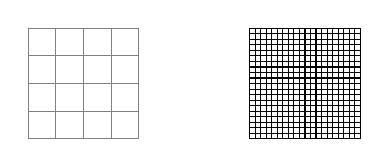
\begin{tikzpicture}[x=40pt,y=40pt]
        \draw[step=10pt,gray] (0,0) grid +(1,1);
        \draw[step=2pt]      (2,0) grid +(1,1);
    \end{tikzpicture}

    \medskip
    % Even though the left grid comes first in English reading order, the right one is much more likely to be seen first: The white-to-black contrast is higher than the gray-to-white contrast. In addition, there are more ``places'' adding to the overall contrast in the right grid.

    即使左边的栅格在英语阅读顺序中排在第一位,右边的栅格也更有可能首先被读者看到:白对黑对比度高于灰对白对比度。 此外,更多的``网格''也增加了右侧网格中的整体对比度。

    % Things like grids and, more generally, help lines usually should not grab the attention of the readers and, hence, should be typeset with a low contrast to the background. Also, a loosely-spaced grid is less distracting than a very closely-spaced grid.

    诸如网格之类的东西,通常是辅助线,通常不应引起读者的注意,因此,其排版应与背景有较低的对比度。 而且,与非常紧密间隔的网格相比,间隔较疏的网格更不会分散注意力。
    % \item Dashed lines create many points at which there is black-to-white contrast. Dashed or dotted lines can be very distracting and, hence, should be avoided in general.
    \item 虚线创建了许多点,这些点之间存在黑白对比。 虚线可能非常分散注意力,因此通常应避免使用。

    %Do not use different dashing patterns to differentiate curves in plots. You lose data points this way and the eye is not particularly good at ``grouping things according to a dashing pattern''. The eye is \emph{much} better at grouping things according to colors.

    不要使用不同的虚线图案来区分图表中的曲线。 您会以这种方式丢失数据点,并且眼睛并不是特别擅长``按照虚线模式对事物进行分组''。 眼睛在根据颜色进行分组方面更胜一筹。
    % \item Background patterns filling an area using  diagonal lines or horizontal and vertical lines or just dots are almost always distracting and, usually, serve no real purpose.
    \item 用斜线、水平线和垂直线或点来填充区域的背景图案几乎总是会分散注意力,而且通常没有真正的作用。
    % \item Background images and shadings distract and only seldomly add anything of importance to a graphic.
    \item 背景图片和阴影分散了注意力,并且很少给图形添加任何重要的东西。
    % \item Cute little clip arts can easily draw attention away from the data.
    \item 可爱的小剪贴画可以很容易地把注意力从数据上转移开来。
\end{itemize}

\clearpage